\documentclass[12pt]{article}
\usepackage{graphicx}
\usepackage[T1]{fontenc}
\usepackage{amsmath}
\usepackage{textcomp}
\usepackage{hyperref}
\usepackage{varioref}
\usepackage{caption} % Pacchetto per modificare la didascalia
\usepackage{subcaption}
\usepackage{authblk}
\captionsetup{font=footnotesize}
\usepackage{tikz}
\usepackage{tabularx}
\usepackage[export]{adjustbox}
\usepackage{placeins}
\usepackage{url}
\usepackage{listings}
\usepackage{xcolor}
\usepackage{mathpazo}
\usepackage{ragged2e}
\hyphenpenalty=5000
\exhyphenpenalty=5000
\renewcommand{\arraystretch}{1.5} % Aumenta l'altezza delle celle
\usepackage{changepage}  % permette adjustwidth
\hypersetup{
    colorlinks,
    linkcolor={black!50!black},
    citecolor={blue!50!black},
    urlcolor={blue!80!black}
}


\title{
\textbf{Esperimento 2} \\[0.5em]
\textbf{Comportamento degli algoritmi con un budget energetico ridotto nei casi limite} \\[1em]
Satellite Computing
}

\author{Claudio Bagini 2045337}
\date{11 Marzo 2026}


\begin{document}
\maketitle


\section{Introduzione}

Nell’ambito del Satellite Computing (SC), il vincolo energetico rappresenta uno dei principali fattori limitanti nella progettazione e nella valutazione delle soluzioni di allocazione delle risorse. A differenza delle infrastrutture terrestri, i satelliti operano infatti in condizioni di disponibilità energetica limitata, rendendo il budget energetico un parametro critico ai fini della sostenibilità operativa del sistema. Il presente esperimento si propone di analizzare l’impatto della riduzione del budget energetico sulla capacità degli algoritmi di \textit{Service Request Assignment} di gestire le richieste di servizio. In particolare, vengono considerate tre configurazioni energetiche per ciascun \textit{Satellite Edge Node} (SEN), pari a $40\,\mathrm{kJ}$, $60\,\mathrm{kJ}$ e $80\,\mathrm{kJ}$, al fine di valutare come tale vincolo influenzi le prestazioni complessive del sistema. Inoltre, l’analisi si concentra su specifiche configurazioni del vettore $B$, che rappresenta la distribuzione delle tipologie di richieste di servizio nel sistema. Oltre a un caso di riferimento standard, vengono considerati tre casi limite, corrispondenti alle configurazioni $B=(0,0,1)$, $B=(0,1,0)$ e $B=(1,0,0)$, in cui l’intero carico di lavoro è composto esclusivamente da una singola tipologia di richiesta. Questa scelta consente di osservare il comportamento degli algoritmi in scenari estremi e di valutare la loro capacità di adattamento a distribuzioni di traffico fortemente sbilanciate.
Gli algoritmi presi in considerazione per questo esperimento sono:

\begin{itemize}
    \item Orbit Aware
    \item DTS
        \begin{itemize}
            \item DTS-Aport
            \item DTS-Base
        \end{itemize}
    \item ILP-Hierarchical
        \begin{itemize}
            \item ILP-Hierarchical-Time
            \item ILP-Hierarchical-Energy
        \end{itemize}
        
\end{itemize}

\section{Esperimento}

Per svolgere questo esperimento mi sono avvalso del simulatore sviluppato dai miei colleghi, che con alcune modifiche mi ha permesso di eseguire tutte le simulazioni necessarie per raccogliere i dati richiesti. In particolare, sono state eseguite complessivamente 360 simulazioni, ottenute combinando i 5 algoritmi sopra elencati con i 3 budget energetici ($40\,\mathrm{kJ}$, $60\,\mathrm{kJ}$ ed $80\,\mathrm{kJ}$) e con le quattro configurazioni del vettore $B$ considerate nell’esperimento, ovvero il caso di riferimento standard $B=(0.4, 0.35, 0.25)$ ed i tre casi limite $B=(0,0,1)$, $B=(0,1,0)$ e $B=(1,0,0)$. Per ciascun budget energetico è stato considerato un tasso di arrivo delle richieste pari a $10$ req/s e, per ogni combinazione di algoritmo, budget energetico e configurazione di $B$, sono stati utilizzati 6 seed diversi, al fine di normalizzare i risultati e ridurre la variabilità statistica. Questa struttura sperimentale ci garantisce un’analisi completa delle prestazioni degli algoritmi sotto differenti condizioni energetiche e diverse distribuzioni del carico di lavoro.


\section{Risultati}

L’analisi dei risultati riportati nelle Tabelle \ref{tab:sr_variation_energy_all} e \ref{tab:rt_st_variation_time_all}, e nei grafici delle Figure~\ref{fig:Grafici}, ~\ref{fig:Grafici-2} e ~\ref{fig:Grafici-3} evidenzia l’impatto del budget energetico sulle prestazioni degli algoritmi di \textit{Service Request Assignment}. In generale, l’aumento dell’energia disponibile produce un incremento della \textit{Success Rate}, con miglioramenti più evidenti nel passaggio da $40\,\mathrm{kJ}$ a $60\,\mathrm{kJ}$ rispetto a quelli osservati tra $60\,\mathrm{kJ}$ e $80\,\mathrm{kJ}$, suggerendo un effetto di progressiva saturazione delle risorse.

Come mostrato nei grafici di \textit{Success Rate} e dei tempi di esecuzione per i diversi budget energetici (Figure~\ref{fig:confronto-algo-40},~\ref{fig:conf-algo-60} e ~\ref{fig:conf-algo-80}), tutti gli algoritmi beneficiano dell’aumento di energia disponibile, poiché i Satellite Edge Node possono gestire un numero maggiore di richieste senza violare i vincoli energetici. Gli algoritmi euristici (\textit{DTS-Aport}, \textit{DTS-Base} e \textit{OrbitAware}) mostrano un comportamento relativamente stabile tra i diversi scenari di traffico, con incrementi generalmente compresi tra circa il $2\%$ e il $3.5\%$ nella \textit{Success Rate} tra $40$ e $60\,\mathrm{kJ}$. Parallelamente, i tempi di risposta (\textit{Response Time}) risultano generalmente contenuti, con valori per immagine compresi tra circa $0.26\,\mathrm{s}$ e $1.27\,\mathrm{s}$, mentre il tempo di sistema (\textit{System Time}) varia tra $0.05\,\mathrm{s}$ e $0.56\,\mathrm{s}$, evidenziando come gli algoritmi euristici riescano a distribuire le richieste senza creare colli di bottiglia eccessivi.

Gli algoritmi basati su ILP, invece, mostrano una maggiore variabilità sia in termini di \textit{Success Rate} sia di tempi di elaborazione. Ad esempio, \textit{ILP-Time} presenta un incremento molto elevato della \textit{Success Rate} nello scenario $B(0,0,1)$ tra $40$ e $60\,\mathrm{kJ}$, ma registra talvolta una diminuzione al passaggio successivo a $80\,\mathrm{kJ}$. Parallelamente, i valori di \textit{Response Time} possono raggiungere fino a $1.45\,\mathrm{s}$ per alcune immagini, mentre il \textit{System Time} oscilla tra $0.07\,\mathrm{s}$ e $0.65\,\mathrm{s}$, evidenziando come gli algoritmi ILP siano più sensibili alle variazioni del carico e della disponibilità energetica.

Infine, l’analisi delle cause di rifiuto (Figure~\ref{fig:conf-rej-40}, \ref{fig:conf-rej-60} e~\ref{fig:conf-rej-80}) mostra come l’aumento del budget energetico riduca progressivamente i rifiuti dovuti al vincolo energetico, rendendo relativamente più rilevanti altre limitazioni del sistema, come i vincoli computazionali o temporali. Questo effetto è coerente con la riduzione dei tempi di risposta per alcune configurazioni, che indica una gestione più efficiente delle richieste da parte dei nodi satellitari.

\begin{table}[h]
\centering
\begin{tabular}{lccc}
\hline
Algorithm & Scenario $B$ & $\Delta SR_{40 \rightarrow 60}$ [\%] & $\Delta SR_{60 \rightarrow 80}$ [\%] \\
\hline

DTS-Aport & B(0.4,0.35,0.25) & 2.88 & 0.82 \\
DTS-Aport & B(0,0,1)         & 3.28 & 0.82 \\
DTS-Aport & B(0,1,0)         & 3.50 & 1.40 \\
DTS-Aport & B(1,0,0)         & 3.55 & 2.64 \\
\hline
DTS-Base & B(0.4,0.35,0.25) & 1.59 & 1.12 \\
DTS-Base & B(0,0,1)         & 2.51 & 1.13 \\
DTS-Base & B(0,1,0)         & 3.75 & 1.19 \\
DTS-Base & B(1,0,0)         & 3.47 & 2.43 \\
\hline
OrbitAware & B(0.4,0.35,0.25) & 2.38 & 2.37 \\
OrbitAware & B(0,0,1)         & 2.99 & 0.68 \\
OrbitAware & B(0,1,0)         & 3.45 & 1.44 \\
OrbitAware & B(1,0,0)         & 3.55 & 2.64 \\
\hline
ILP-Time & B(0.4,0.35,0.25) & 1.44 & 2.60 \\
ILP-Time & B(0,0,1)         & 9.68 & -1.09 \\
ILP-Time & B(0,1,0)         & 0.37 & -0.78 \\
ILP-Time & B(1,0,0)         & 1.41 & -0.77 \\
\hline
ILP-Energy & B(0.4,0.35,0.25) & -0.82 & 2.24 \\
ILP-Energy & B(0,0,1)         & 2.88 & 0.39 \\
ILP-Energy & B(0,1,0)         & -0.31 & 2.38 \\
ILP-Energy & B(1,0,0)         & 1.91 & -1.55 \\

\hline
\end{tabular}
\caption{Variazione della Success Rate (\%) al crescere del budget energetico per ciascun algoritmo e scenario $B$.}
\label{tab:sr_variation_energy_all}
\end{table}
\FloatBarrier

\begin{table}[h]
\centering
\small
\setlength{\tabcolsep}{0.0000001pt}
\begin{tabularx}{\textwidth}{lXcccccc}
\hline
Algorithm & Scenario $B$ 
& $\Delta RT_{40 \rightarrow 60}$ [\%] 
& $\Delta RT_{60 \rightarrow 80}$ [\%]
& $\Delta ST_{40 \rightarrow 60}$ [\%]
& $\Delta ST_{60 \rightarrow 80}$ [\%] \\
\hline
DTS-Aport      & B(0.4,0.35,0.25) & 0.17 & 0.93 & 0.25 & 1.09 \\
DTS-Aport      & B(0,0,1)         & 1.14 & 0.85 & 1.39 & 0.76 \\
DTS-Aport      & B(0,1,0)         & 2.35 & 0.34 & 2.84 & 0.44 \\
DTS-Aport      & B(1,0,0)         & -0.27 & 0.00 & 0.17 & 0.00 \\
\hline
DTS-Base       & B(0.4,0.35,0.25) & 1.08 & -0.34 & 1.28 & -0.52 \\
DTS-Base       & B(0,0,1)         & 2.44 & -0.14 & 2.71 & -0.11 \\
DTS-Base       & B(0,1,0)         & 2.37 & 0.16 & 2.71 & 0.21 \\
DTS-Base       & B(1,0,0)         & -0.19 & 0.04 & 0.35 & 0.17 \\
\hline
OrbitAware     & B(0.4,0.35,0.25) & 0.29 & 1.76 & 0.25 & 2.23 \\
OrbitAware     & B(0,0,1)         & 1.71 & 0.56 & 1.96 & 0.49 \\
OrbitAware     & B(0,1,0)         & 2.27 & 0.39 & 2.80 & 0.48 \\
OrbitAware     & B(1,0,0)         & -0.27 & 0.00 & 0.17 & 0.00 \\
\hline
ILP-Time       & B(0.4,0.35,0.25) & 1.25 & 1.90 & 1.46 & 2.19 \\
ILP-Time       & B(0,0,1)         & 2.75 & 0.20 & 3.08 & 0.34 \\
ILP-Time       & B(0,1,0)         & 7.95 & -0.85 & 8.91 & -1.02 \\
ILP-Time       & B(1,0,0)         & -1.10 & 1.12 & -3.41 & 2.68 \\
\hline
ILP-Energy     & B(0.4,0.35,0.25) & 7.56 & -0.53 & 9.05 & -0.53 \\
ILP-Energy     & B(0,0,1)         & 0.93 & 2.20 & 0.80 & 2.49 \\
ILP-Energy     & B(0,1,0)         & 4.24 & 2.41 & 4.82 & 2.65 \\
ILP-Energy     & B(1,0,0)         & 0.98 & -1.13 & 2.36 & -2.44 \\
\hline
\end{tabularx}
\caption{Variazione percentuale del Response Time e System Time al crescere del budget energetico per ciascun algoritmo e scenario $B$.}
\label{tab:rt_st_variation_time_all}
\end{table}
\FloatBarrier

\begin{figure}[p]
\begin{adjustwidth}{-5cm}{-5cm}  % estende 2cm a sinistra e 2cm a destra
    \centering
    % --- Prima riga ---
    \begin{subfigure}[b]{0.70\textwidth}
        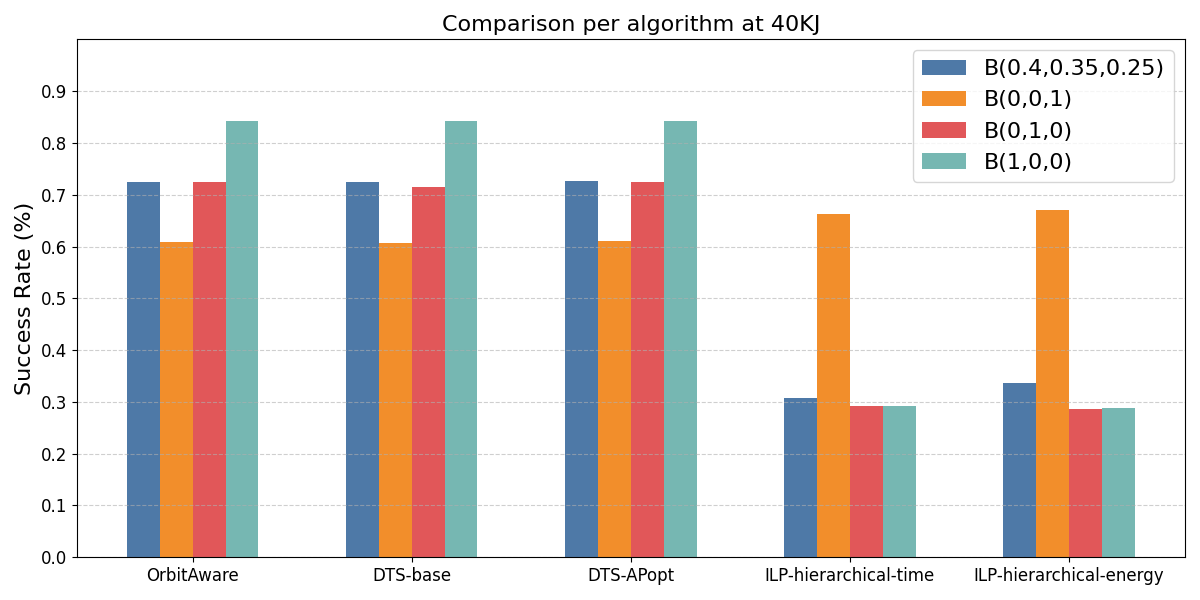
\includegraphics[width=\textwidth,height=0.32\textheight,keepaspectratio]{comparison_algos_40000.png}
        \caption{Success rate con 40\,kJ}
        \label{fig:confronto-algo-40}
    \end{subfigure}
    \hspace{0.02\textwidth}
    \begin{subfigure}[b]{0.70\textwidth}
        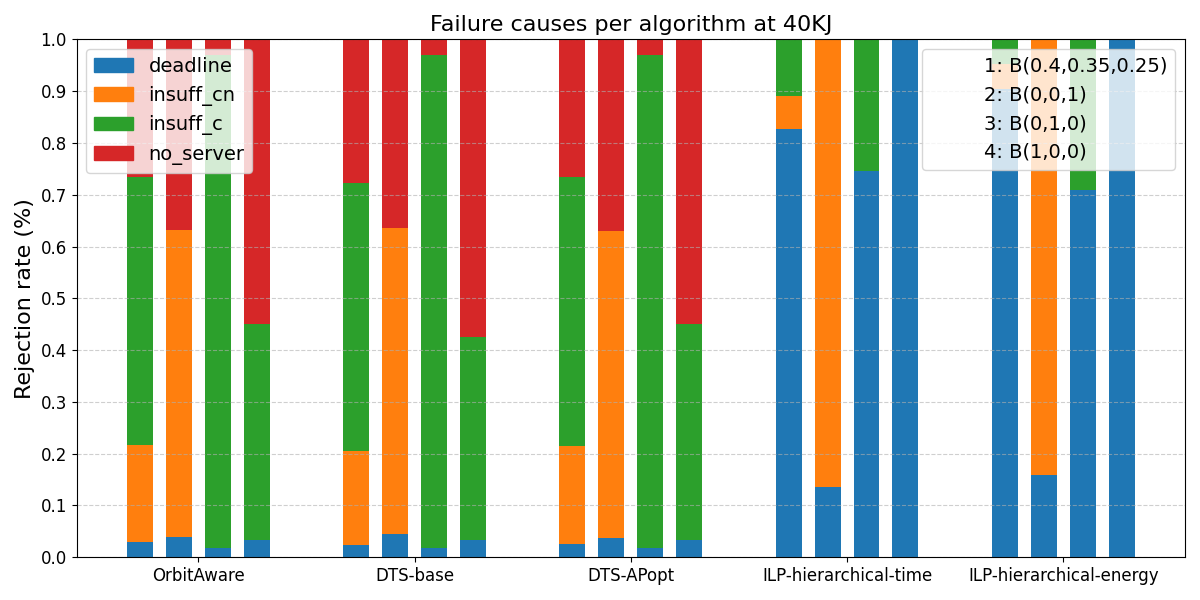
\includegraphics[width=\textwidth,height=0.32\textheight,keepaspectratio]{rejection_causes_40000.png}
        \caption{Rejection causes con 40\,kJ}
        \label{fig:conf-rej-40}
    \end{subfigure}

    \vspace{0.5em}

    % --- Seconda riga ---
    \begin{subfigure}[b]{0.70\textwidth}
        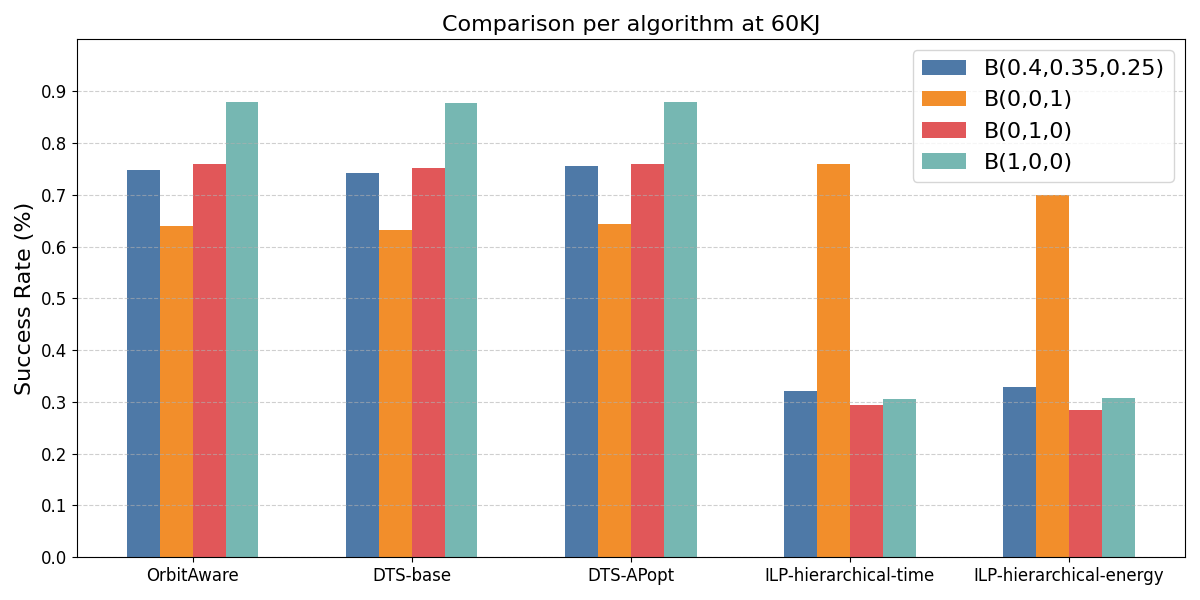
\includegraphics[width=\textwidth,height=0.32\textheight,keepaspectratio]{comparison_algos_60000.png}
        \caption{Success rate con 60\,kJ}
        \label{fig:conf-algo-60}
    \end{subfigure}
    \hspace{0.02\textwidth}
    \begin{subfigure}[b]{0.70\textwidth}
        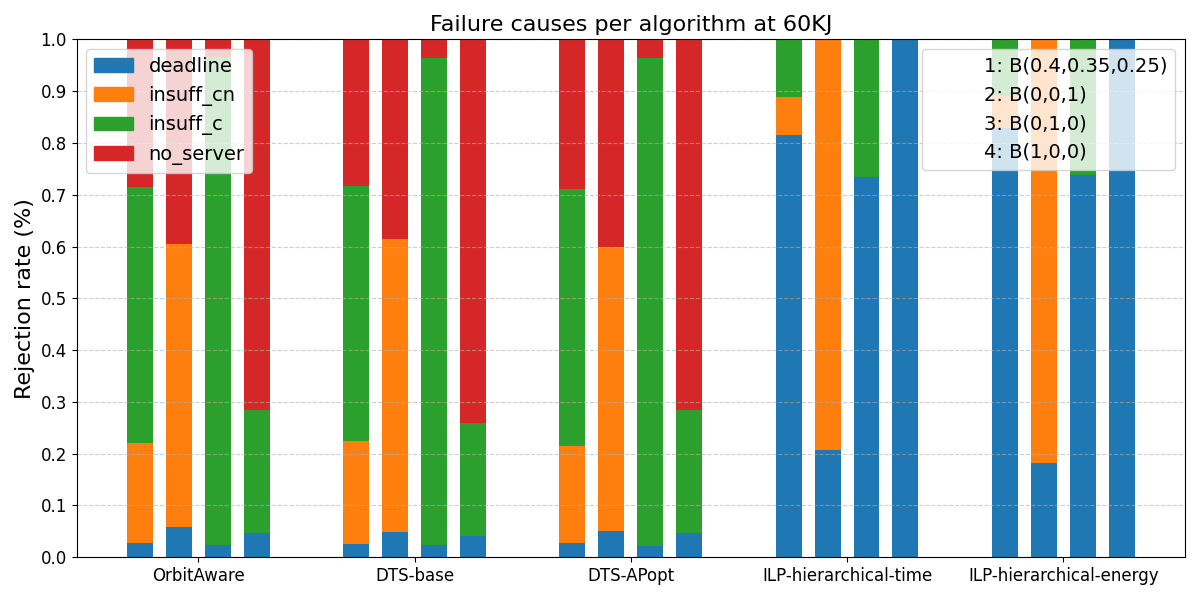
\includegraphics[width=\textwidth,height=0.32\textheight,keepaspectratio]{rejection_causes_60000.png}
        \caption{Rejection causes con 60\,kJ}
        \label{fig:conf-rej-60}
    \end{subfigure}

    \vspace{0.5em}

    % --- Terza riga ---
    \begin{subfigure}[b]{0.70\textwidth}
        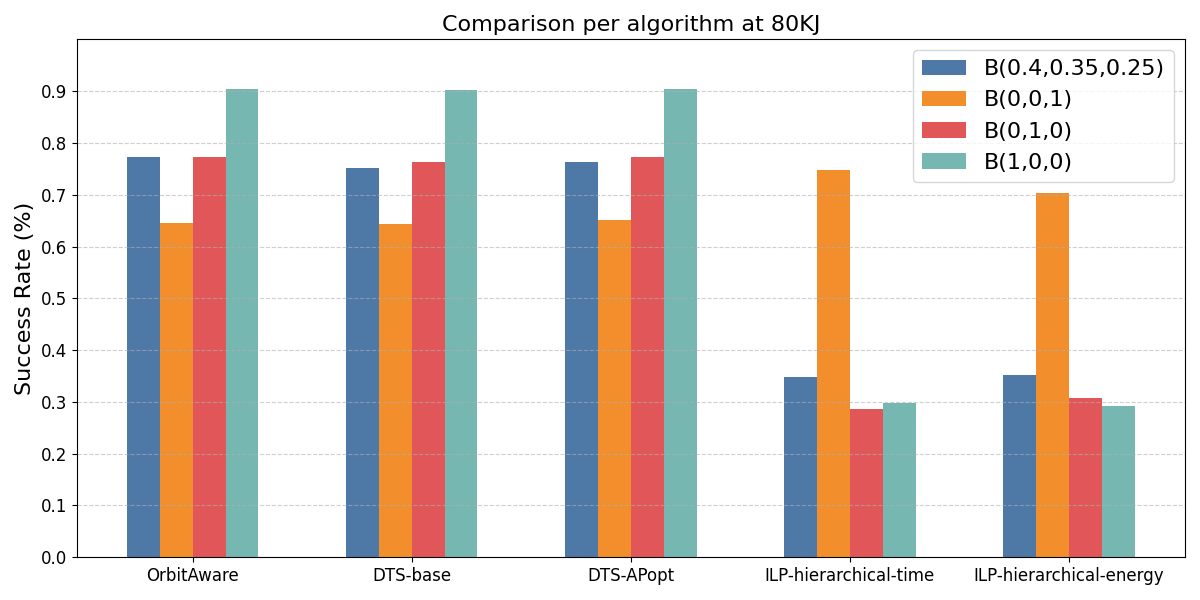
\includegraphics[width=\textwidth,height=0.32\textheight,keepaspectratio]{comparison_algos_80000.png}
        \caption{Success rate con 80\,kJ}
        \label{fig:conf-algo-80}
    \end{subfigure}
    \hspace{0.02\textwidth}
    \begin{subfigure}[b]{0.70\textwidth}
        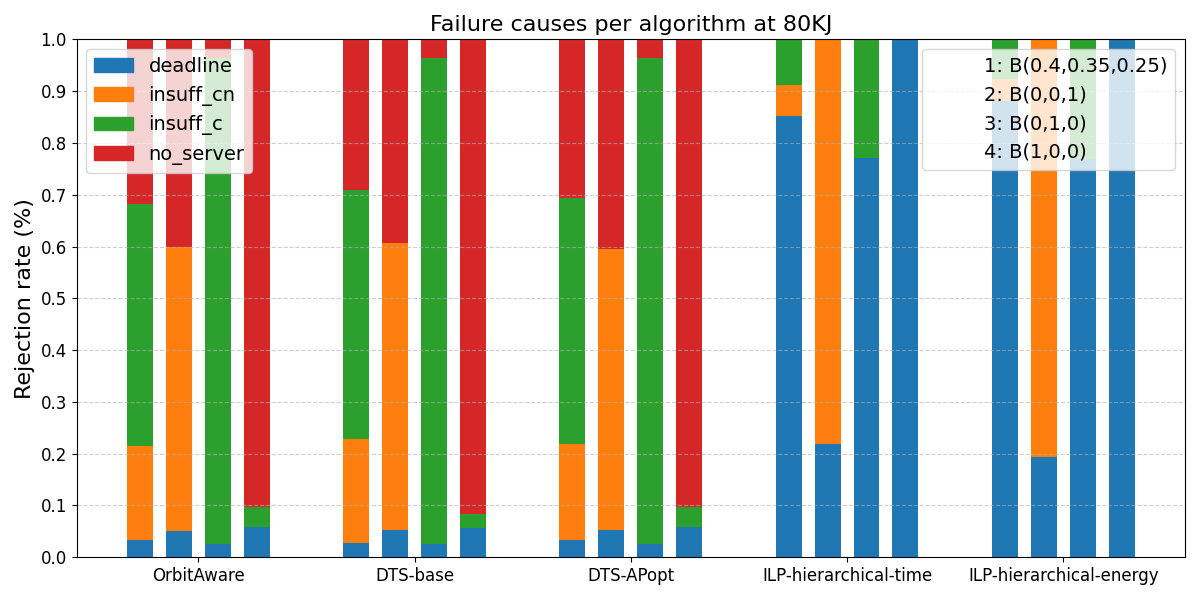
\includegraphics[width=\textwidth,height=0.32\textheight,keepaspectratio]{rejection_causes_80000.png}
        \caption{Rejection causes con 80\,kJ}
        \label{fig:conf-rej-80}
    \end{subfigure}

    \caption{Grafici dei risultati sperimentali} 
    \label{fig:Grafici}
\end{adjustwidth}
\end{figure}
\FloatBarrier


\begin{figure}[p]
\begin{adjustwidth}{-5cm}{-5cm}  % estende 2cm a sinistra e 2cm a destra
    \centering
    % --- Prima riga ---
    \begin{subfigure}[b]{0.70\textwidth}
        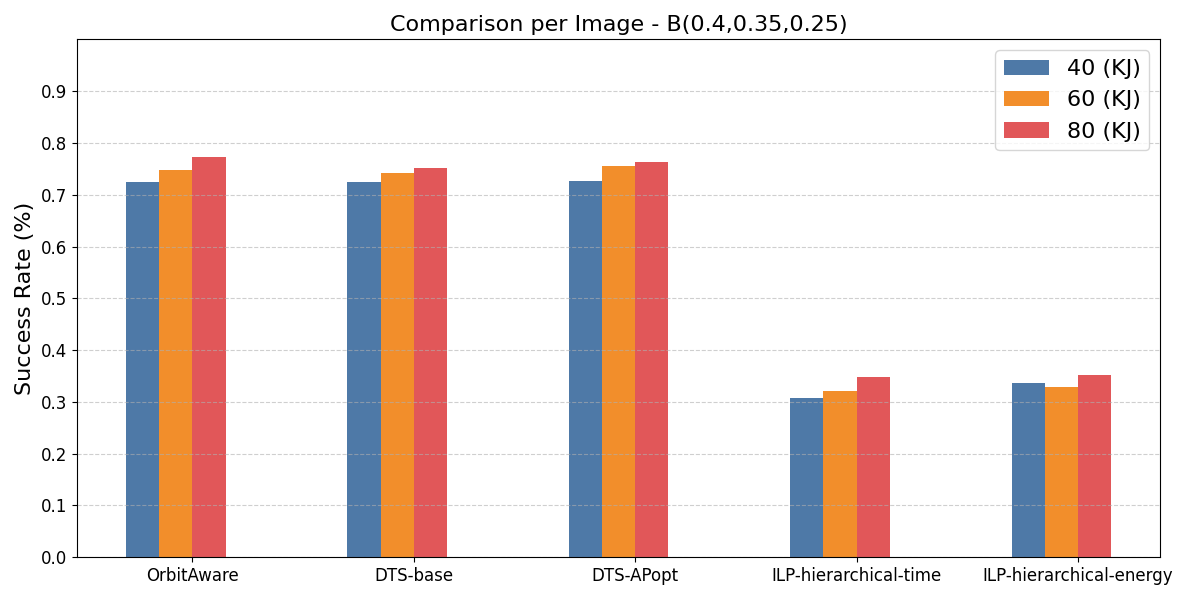
\includegraphics[width=\textwidth,height=0.32\textheight,keepaspectratio]{comparison_algos_img_0.45_0.35_0.25.png}
        \caption{Success rate con B(0.4, 0.35, 0.25)}
        \label{fig:conf-im-04}
    \end{subfigure}
    \hspace{0.02\textwidth}
    \begin{subfigure}[b]{0.70\textwidth}
        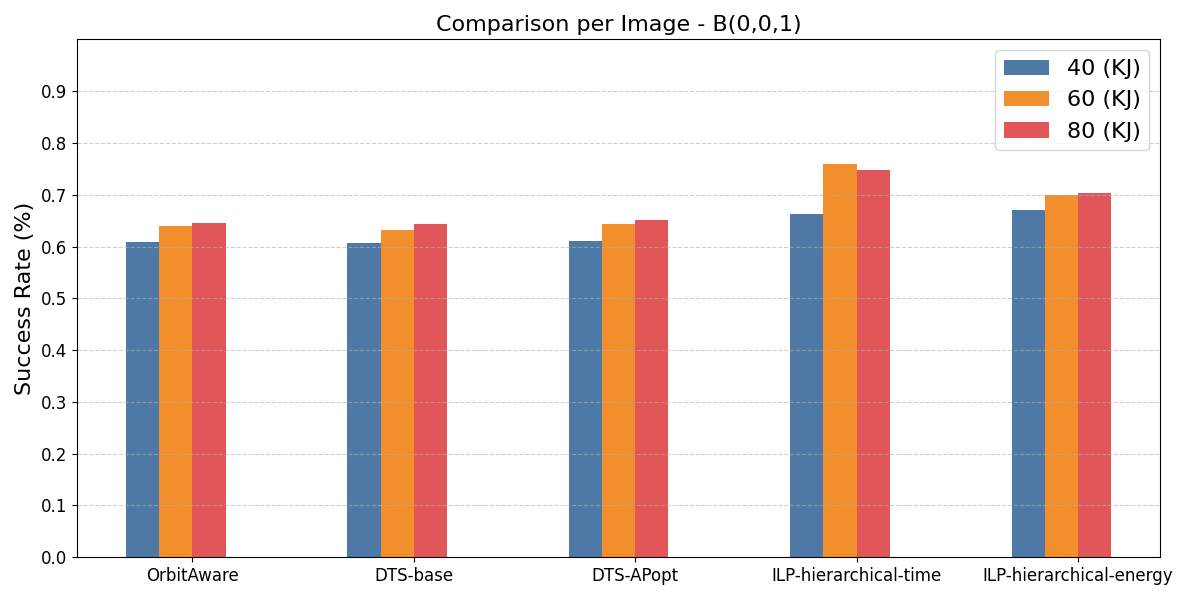
\includegraphics[width=\textwidth,height=0.32\textheight,keepaspectratio]{comparison_algos_img_0_0_1.png}
        \caption{Success rate con B(0, 0, 1)}
        \label{fig:conf-im-001}
    \end{subfigure}

    \vspace{0.5em}

    % --- Seconda riga ---
    \begin{subfigure}[b]{0.70\textwidth}
        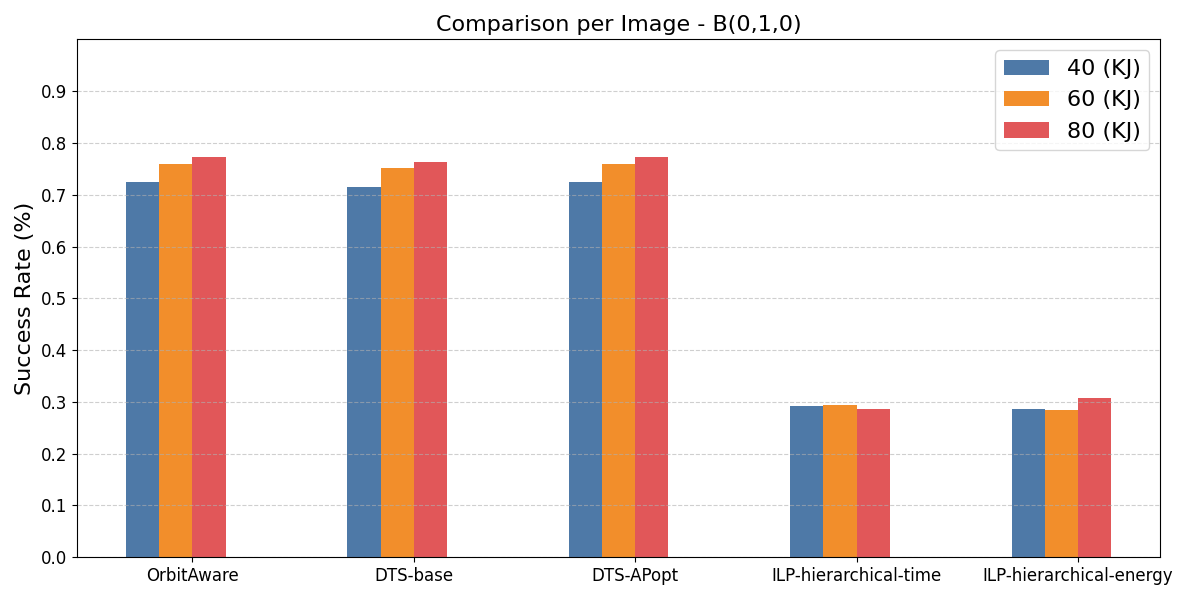
\includegraphics[width=\textwidth,height=0.32\textheight,keepaspectratio]{comparison_algos_img_0_1_0.png}
        \caption{Success rate con B(0, 1, 0)}
        \label{fig:conf-im-010}
    \end{subfigure}
    \hspace{0.02\textwidth}
    \begin{subfigure}[b]{0.70\textwidth}
        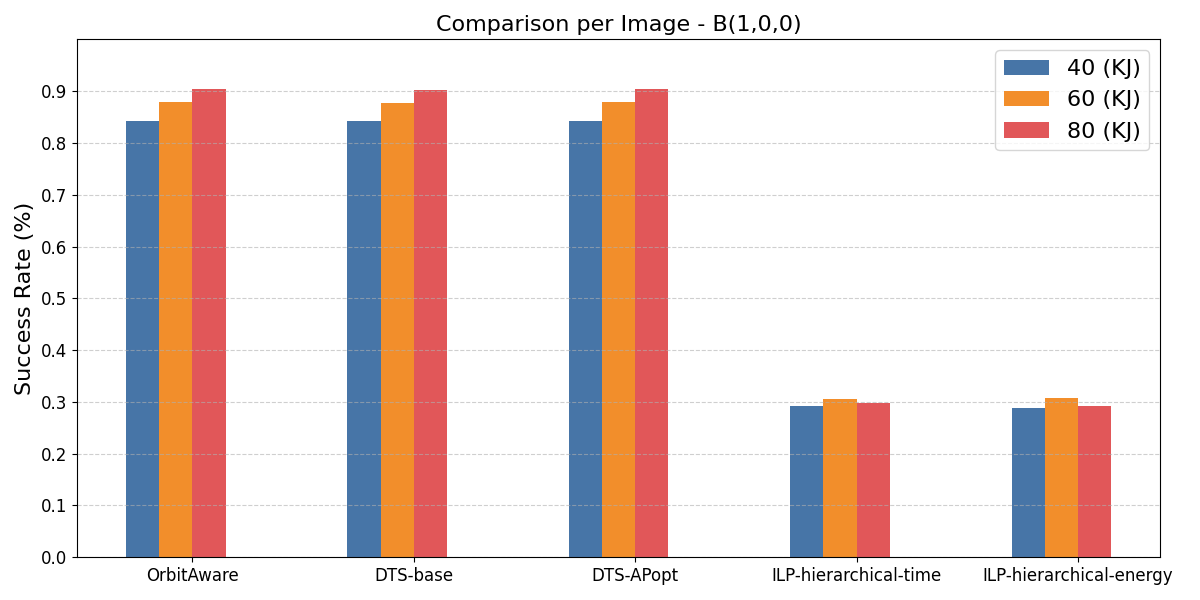
\includegraphics[width=\textwidth,height=0.32\textheight,keepaspectratio]{comparison_algos_img_1_0_0.png}
        \caption{Success rate con B(1, 0, 0)}
        \label{fig:conf-im-100}
    \end{subfigure}

    \vspace{0.5em}
        % --- Terza riga ---
    \begin{subfigure}[b]{0.70\textwidth}
        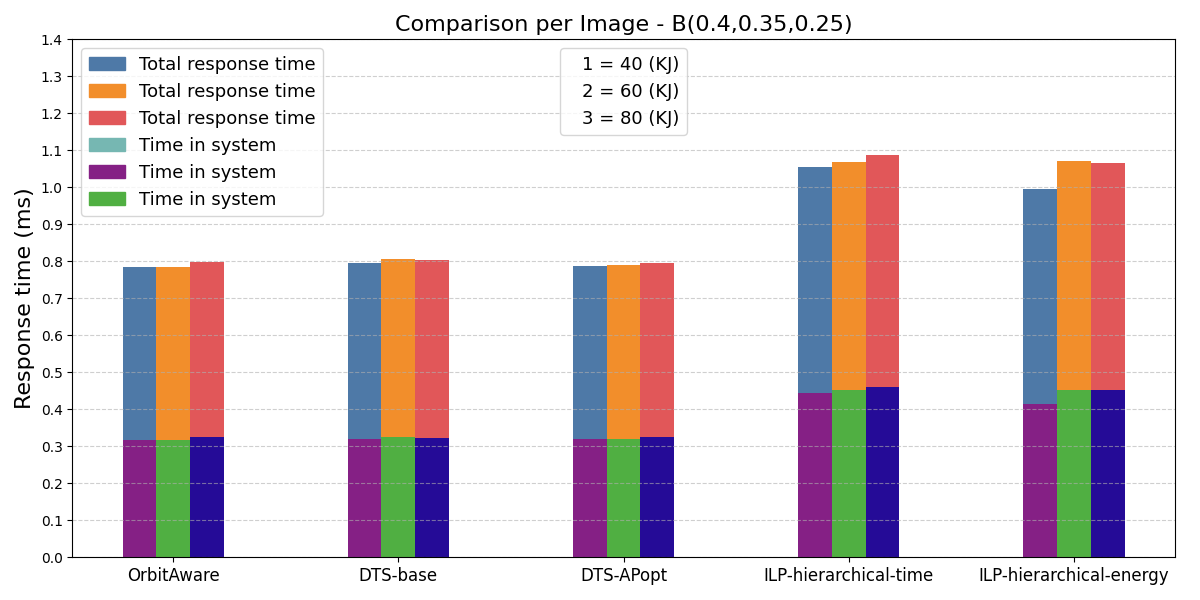
\includegraphics[width=\textwidth,height=0.32\textheight,keepaspectratio]{comparison_response_time_img_0.45_0.35_0.25.png}
        \caption{Response time con B(0.4, 0.35, 0.25)}
        \label{fig:conf-re-0.4}
    \end{subfigure}
    \hspace{0.02\textwidth}
    \begin{subfigure}[b]{0.70\textwidth}
        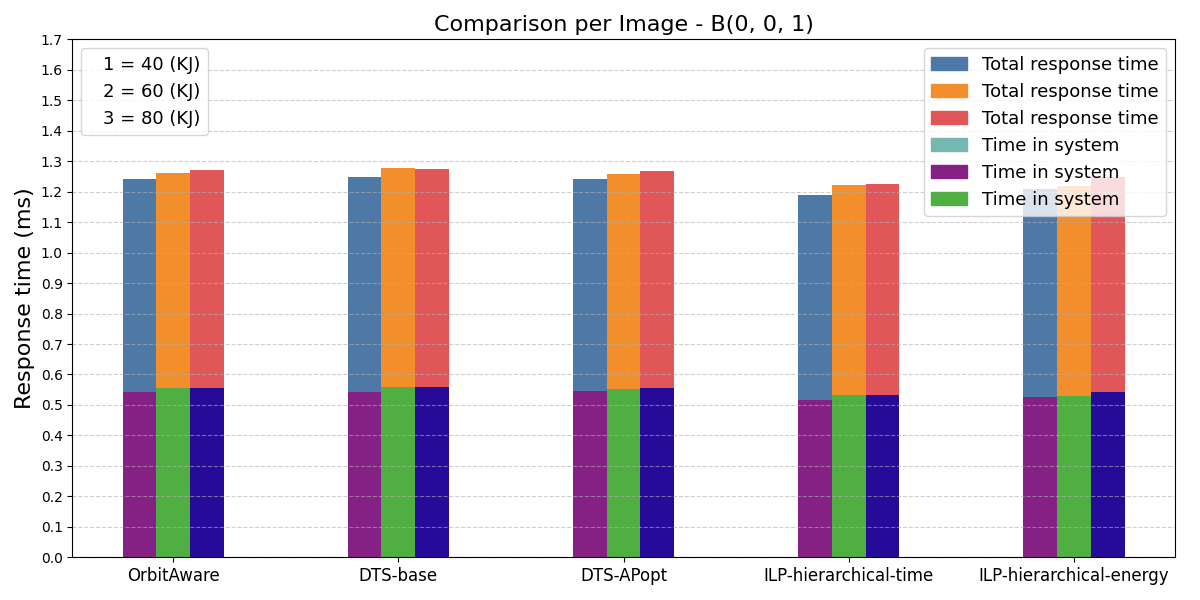
\includegraphics[width=\textwidth,height=0.32\textheight,keepaspectratio]{comparison_response_time_img_0_0_1.png}
        \caption{Response Time con B(0, 0, 1)}
        \label{fig:conf-re-001}
    \end{subfigure}

    \caption{Grafici dei risultati sperimentali} 
    \label{fig:Grafici-2}
\end{adjustwidth}
\end{figure}
\FloatBarrier

\begin{figure}[h]
\begin{adjustwidth}{-5cm}{-5cm}  % estende 2cm a sinistra e 2cm a destra
    \centering
    % --- Prima riga ---
    \begin{subfigure}[b]{0.70\textwidth}
        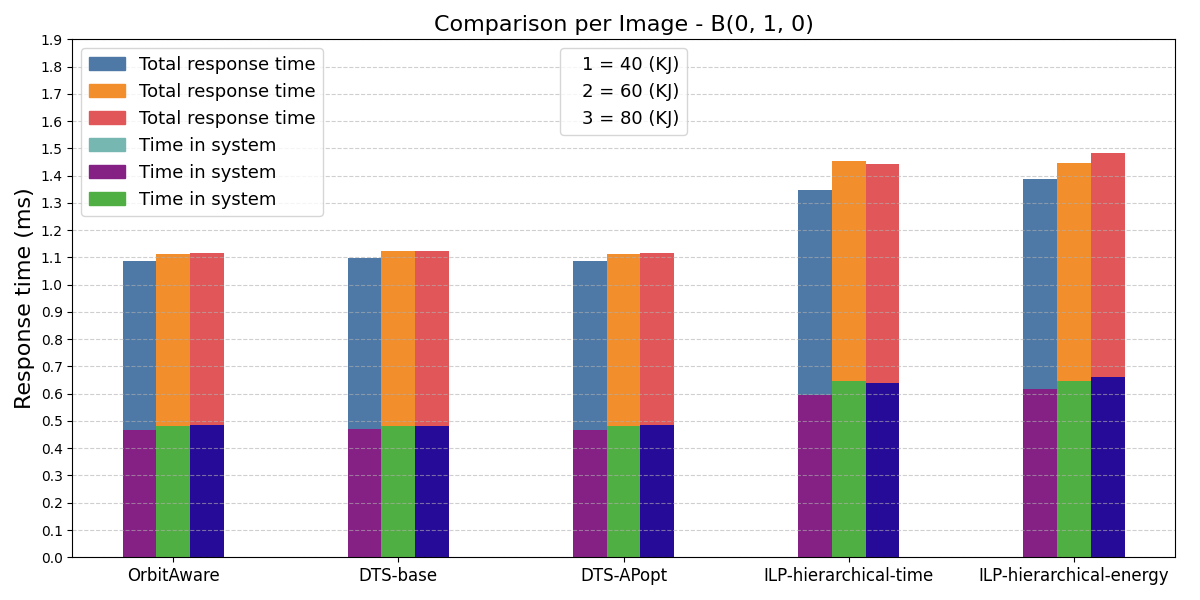
\includegraphics[width=\textwidth,height=0.32\textheight,keepaspectratio]{comparison_response_time_img_0_1_0.png}
        \caption{Response time con B(0, 1, 0)}
        \label{fig:conf-re-010}
    \end{subfigure}
    \hspace{0.02\textwidth}
    \begin{subfigure}[b]{0.70\textwidth}
        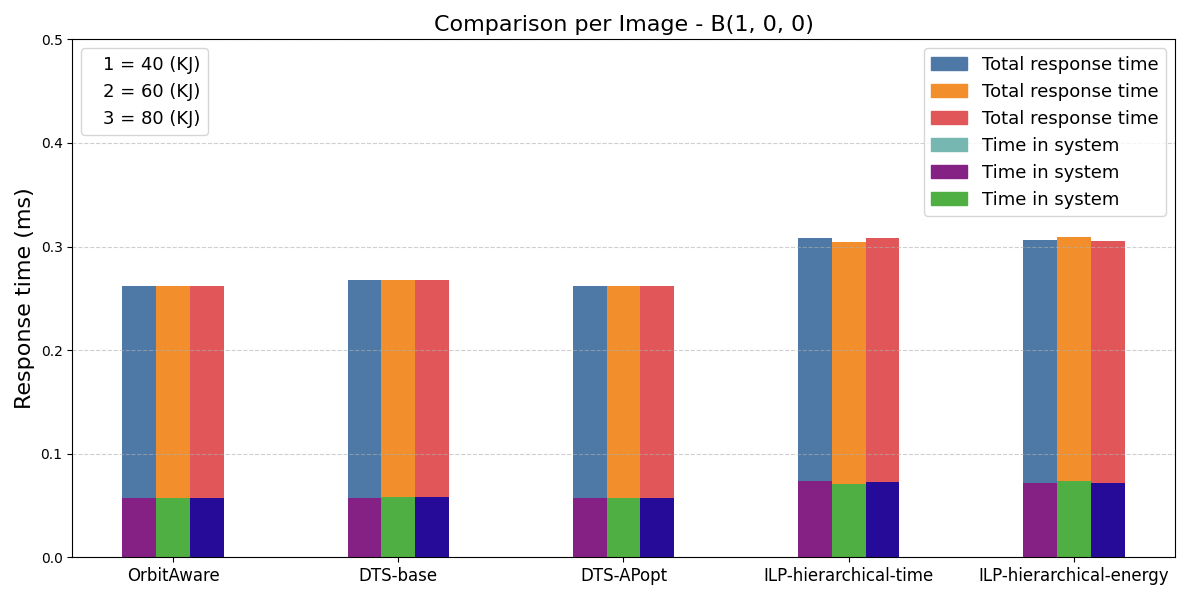
\includegraphics[width=\textwidth,height=0.32\textheight,keepaspectratio]{comparison_response_time_img_1_0_0.png}
        \caption{Response time con B(1, 0, 0)}
        \label{fig:conf-re-100}
    \end{subfigure}

    \caption{Grafici dei risultati sperimentali} 
    \label{fig:Grafici-3}
\end{adjustwidth}
\end{figure}
\FloatBarrier

\section{Conclusione}

In conclusione, l’esperimento ha permesso di analizzare in modo sistematico l’impatto del vincolo energetico sulle prestazioni degli algoritmi di \textit{Service Request Assignment} nel contesto del Satellite Computing. La valutazione su diversi budget energetici e su differenti configurazioni del vettore $B$ ha consentito di osservare il comportamento degli algoritmi sia in condizioni operative bilanciate sia in scenari limite, in cui il carico di lavoro è concentrato su una singola tipologia di richiesta. I risultati ottenuti forniscono quindi indicazioni utili sulla robustezza e sulla capacità di adattamento delle diverse strategie di allocazione delle risorse in presenza di forti vincoli energetici.


\end{document}